\section{Revised Block Diagram}

Figure~\ref{fig:blockDiagram} shows a revised system block diagram.  It contains the model numbers of the known components, the type of connection required to the microcontroller unit and the amount of lines needed for each connection.  Several components such as the power management circuit, battery meter and charger are still to be chosen as several methods of battery charging are being considered.

%TODO Fix amount of lines in block diagram
\begin{figure}[H]
	\centering
	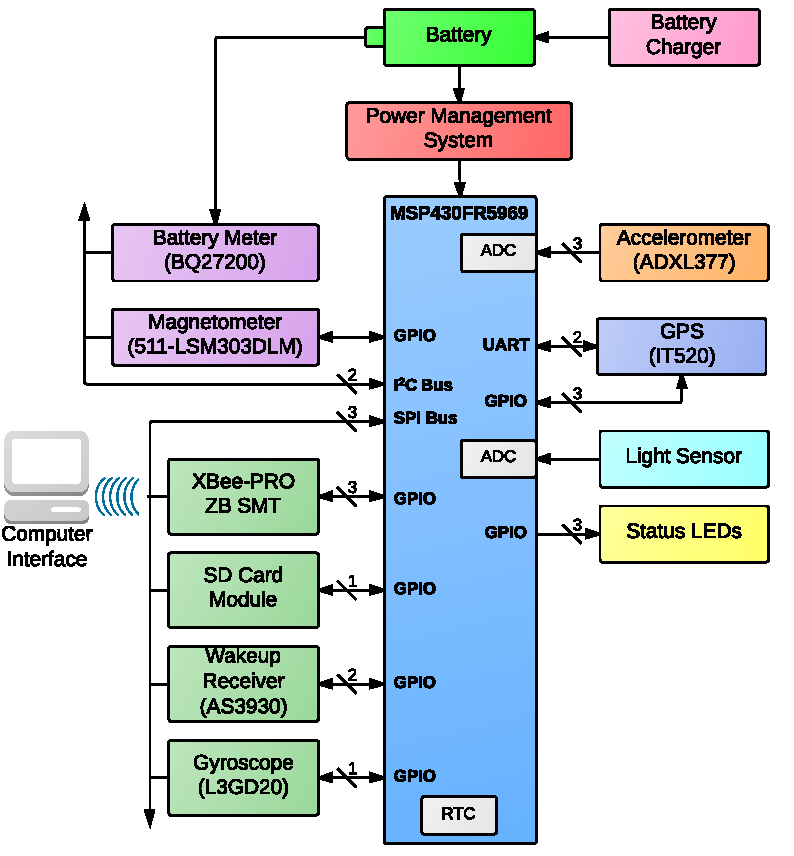
\includegraphics[width=\textwidth]{img/blockDiagramV2_2}
	\caption{Revised Block Diagram \label{fig:blockDiagram}}
\end{figure}

\subsection{RF Wake-Up Receiver}
The RF Wake-Up receiver is a dedicated component that is utilized to interrupt and wake the MCU from low power mode while consuming very low power listening for the wake-up signal. This enables the device to power on without the need of an external physical button. It also enables the device to operate in Shutdown Mode, where very little power is being consumed waiting for user interaction.

\subsection{Battery Charging Methods}
Two different methods are being considered for charging the sphere's battery.
\subsubsection{USB Charger}
Big effort has been made in recent years to standardize chargers and connectors for music players, cellphones, tablets, and many other consumer electronic products. Micro USB has taken the lead as the standard port for charging consumer electronics and manufacturers have dropped their own proprietary connectors to favor the USB standard.

The USB 2.0 standard included the Battery Charging Specification 1.2, which increased the limits of supply current to 1.5A, up from the 500mA the USB 1.0 standard allowed. The USB 3.0 specification allows 900mA of current drawn while concurrently transmitting data. For battery charging, the limit is still 1.5A, even though the Battery Charging specification requires the physical ports themselves to be able to handle 5A.

There are many variables in question when it comes to choosing a battery charger. Different battery technologies need to be charged distinctively. For this application, a technology such as Lithium-Ion or Lithium-Polymer must be used, because Lead-Acid, Nickel-Cadmium, and Nickel-Metal-Hydride batteries are too big, heavy, and do not provide the necessary voltage for this application. It is for this reason also that Li-Ion and Li-Polymer batteries are chosen for most consumer electronics.

Other variables include the number of battery cells that need to be charged and the kind of topology needed to charge the battery. For Lithium-Ion and Lithium-Polymer, two topologies exist: Linear and Switch-mode.

Most handheld devices use a linear charging topology, because it offers many advantages like low implementation cost, design simplicity, and a non-noisy operation because it has no high frequency switching components. One of the drawbacks of this topology is that it introduces power dissipation in the system. Switch-mode topology offers higher efficiency, but the implementation is more complicated, bulkier, and noisy, which may cause interference. For this application, a linear charging topology is preferred.

After having decided the implementation variables, a charge management controller should be chosen. There are many controllers available commercially. A good example is Microchip's MCP73831/2. This is a single cell, fully integrated Li-Ion and Li-Polymer charge management controller. It uses a linear topology and it is compatible with the standard Micro USB port. 

Another good example is Texas Instrument's bq24080. It also uses a linear charge topology, and contains a status indicator pin.
\subsubsection{Wireless Charger}
Wireless charging involves charging the sphere's battery without being physically connected to an outlet or to another device. The reason this method is being considered is because if the device is wirelessly charged then the device wouldn't need an external port that would be use to charge the device without opening the sphere and if no external port is used then it wouldn't also be needed for the user to physically open the sphere and disconnect the battery to charge it somewhere else. 

Exploring the idea we discovered the Qi (pronounced \'chee\') standard which dictates a wireless charging and communication interface. Qi standards mention that the energy transfer must occur to a distance up to 40 millimeters and that the primary inductive coil must be flat in a spiral formation \cite{QiStandard}. With such constrains the Qi standard is discarded and because furthermore the standard is intended to be used for multiple devices with different power requirements, Qi has a communication protocol that complicate the devices and obligates us to integrate further IC that can potentially use space. Discarding Qi lead us to consider implementing a custom wireless charger, the idea is to basically transfer energy from a 120V AC outlet trough a transformer into the spheres. The transformer will actually be two separated coils which by inductance can transfer energy at a long distance. An AC current will be created inside the sphere's coil which will then have to be rectified into a DC current that can charge the device's battery. Various factors are to be considered when implementing such charger, energy transferring by inductance is not very efficient, the coils require specific geometry and number of turns, moreover the frequency in which the current changes in the primary coil must be specific, such ideal resonance frequency is needed to archive maximum energy transfer. 

Research and experiments are being performed to converge into an implementation, it is possible to supply the primary coil with a controlled oscillating DC current that would still cause the necessary change in flux to create an inductive charge. Ideally the user will have a charge station that will be connected to a power outlet and can hold a few spheres, each sphere being hold by such charging station is being charged wirelessly without the need of connecting it or opening it. 
